% Every document starts with the declaration of the type of document,
% for example report, book, beamer (for presentation like the ones in
% these seminars), standalone, ...
% In LaTeX every command starts with /, arguments are supplied inside {}
% and optional arguments inside []

% A LaTeX document is composed by two parts: the preable, where the used
% packages and the options are defined, and the main body, where is the
% actual test

% Report is for reports
\documentclass[12pt]{report}

% To import images
\usepackage{graphicx}

% The draw plots
\usepackage{pgfplots}
\usetikzlibrary{shapes}

% The typeset units
\usepackage{siunitx}

% Add maths symbols and math functions
\usepackage{amsmath}
\usepackage{amsthm}
\usepackage{amssymb}

% Language hyphenation and typographical rules
\usepackage[english]{babel}

% For urls and href
\usepackage{hyperref}

% Define definition and theorem env
\newtheorem{definition}{Definition}
\newtheorem{theorem}{Theorem}

% I can define personal macros and envs
\newcommand{mysign}{\emph{Garbiele Bozzola}}

% Set up some metadata

% The \\ symbol means newline

\author{%
\textsc{Gabriele Bozzola}\thanks{\href{mailto:bozzola.gabriele@gmail.com}{bozzola.gabriele@gmail.com}} \\[1ex]
\normalsize Universit\'a degli Studi di Milano \\
\normalsize
}
\date{\today}
\title{Simulation of dice rolls}


% The begin document statement ends the preable and stars the main body
\begin{document}

% Print the title page
\maketitle

% The statements begin{} and end{} define an environment
% Environments are used for figures, tables, text formatting, equations..

\begin{abstract}
  In this work numerical simulation are used for verifying the law of large
  numbers \cite{lawoflarge} and the central limit theorem.
\end{abstract}

% Print the table of contents
\tableofcontents

% To start a new chapter, LaTeX takes care about numbering. If you don't
% want the chapter to be in the toc just use chapter*
% Available sectioning are: part > chapter > section > subsection > subsubsection > paragaph > subparagraph

\chapter{Mathematical Introduction}

% To print a mathematica formula inline use $ $, to print it in a new line \[ \], or
% eqution if you want the numbering

This is simple text.           Multiple spaces are treated as only one.

A single empty line means nothing.


Two or more empty lines means newline.

{\Large graphs define scopes.}


\section{Definitions}

% textbf, emph, mathbb, mathrm, text are all text modifier (bold text, italic, ...)
\begin{definition}
A \textbf{$N$-faced die} is the set $\{ n \in \mathbb{N} \text{ with } n \leq N \}$.
\end{definition}

Please, typeset units with siunitx: $\SI{1.5e4}{\m\per\s}$.

\section{Theorems}

\begin{theorem}
  The \textbf{expected value} of a $N$-faced die is:

% The equation environment is like the \[ \] but it is also numbered
% Moreover, it is possible to attach a label to the equation, so that
% it is possible to refer to this equation without knowing the number
  \begin{equation}
    \label{eq:exp_value}
    \mathrm{Exp}[N] = \frac{\sum_{i = 1}^N i}{N}
  \end{equation}
  % It is customary to label equations starting with eq:, figures with
  % fig:, tables with tab: and sections with sec:
\end{theorem}
\begin{proof}
  Assuming that each face has the same probability the expected value
  is obtained with an arithmetic mean, which is exactly \eqref{eq:exp_value}.
\end{proof}
\begin{theorem}[The law of large numbers]
  The average value of $N$ die rolls goes to the expected value if $N\to\infty$.\end{theorem}
\begin{proof}
  The proof is left as useful exercise to the reader.
\end{proof}
\begin{theorem}[The central limit theorem]
  If $d1$, $d2$ are two dice $N$-rolls, and $s$ is the sum of the results of
  $d1$ and $d2$, then $s$ is a Gaussian if $N\to\infty$.
\end{theorem}
\begin{proof}
  Trivial.
\end{proof}

\chapter{Results}
\label{cha:results}

\section{The law of large numbers}
\label{sec:law-large-numbers}

The law of large numbers is verified:%
% The figure environment tells LaTeX that it has to treat the figure
% as a floating item, which means that LaTeX is allowed to move it according its typographical taste.

\LaTeX has a powerful packages for drawing plots.

\begin{figure}[htbp]
  \centering
  \begin{tikzpicture}
    \begin{axis}[
      width=\linewidth, % Scale the plot to \linewidth
      height=0.67\linewidth, % Scale the plot to \linewidth
      grid=major, % Display a grid
      grid style={dashed,gray!30}, % Set the style
      xlabel=Roll number, % Set the labels
      ylabel=Value,
      legend style={at={(0.8,0.2)},anchor=north},
      ]
      \addplot table {aver.dat};
      \addlegendentry{Average value}
      \addplot[mark=none, red, samples=2, domain=0:5000,
      line width = 4] {4.5};
      \addlegendentry{Expected value}
    \end{axis}
  \end{tikzpicture}
  \caption{The law of large numbers}
  \label{fig:largenumbers}
\end{figure}

% Tikzpicture can be used also for diagrams, maps or simple drawings
% http://www.texample.net/tikz/examples/ contains many examples

\begin{figure}[htbp]
  \centering
  
\begin{tikzpicture}
    \draw[very thick, rounded corners] (0,0) rectangle (1,1);
    \node[ellipse,fill=black,minimum height=0.1em] at (0.5,0.5){};
  \end{tikzpicture}
  \caption{A simple die}
  \label{fig:die}
\end{figure}

\section{The central limit theorem}
\label{sec:centr-limit-theor}

\begin{figure}[htbp]
  % htbp = here top bottom page
  % If possible put here, if not put on the top, if not put on the bottom, if
  % not put on another page
  % Center the figure
  \centering
  % Include the figure (better use always vectors not rasters!)
  % width=\textwidth fixes the width to be the same of the text
  % The height is rescaled to keep the ratio
  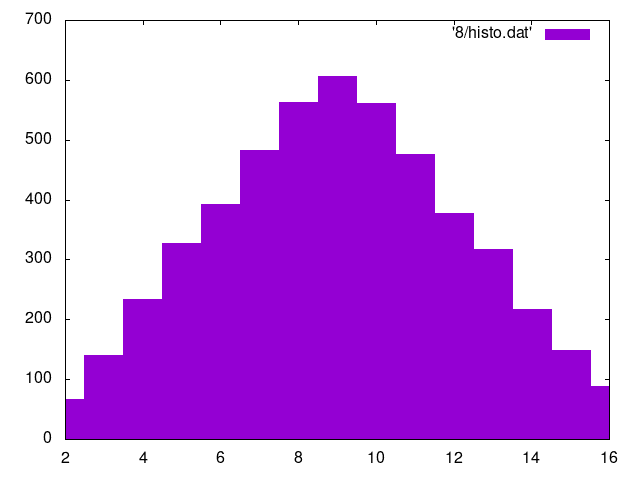
\includegraphics[width=0.8\textwidth]{images/histo.png}
  % Add a caption
  \caption{The central limit theorem}
  \label{fig:clt}
\end{figure}
% Tables are the floating environment that contains tabular, which is
% the actual table
\begin{table}[htbp]
  \centering
  % In table caption should be placed above the content
  \caption{Some data}
  \bigskip
  \label{tab:somedata}
  % The ampersand symbol defines new columns, the \\ new rows
  \begin{tabular}[htbp]{c|c}
    Roll number & Value \\ \hline
    1           & 4     \\
    2           & 8     \\
    3           & 2     \\
    \dots           & \dots
  \end{tabular}
\end{table}

% This is the most basic way to produce a bibliography, but for larger documents
% usually biblatex is used. With biblatex one writes a library of references and
% include the library in the tex file, then cites only what he wants to cite.
% The biblatex entries can be downloaded and usually are not typed manually

\begin{thebibliography}{9}
\bibitem{lawoflarge}
Feller, W. \emph{The Strong Law of Large Numbers}. §10.7 in An Introduction to
Probability Theory and Its Applications, Vol. 1, 3rd ed. New York: Wiley, pp.
243-245, 1968.
\end{thebibliography}

\end{document}

%%% Local Variables:
%%% mode: latex
%%% TeX-master: t
%%% End:
